\section{Módulo Android}

O módulo Android do sistema é responsável pela visualização dos dados referentes a um
determinado paciente e também pela notificação do usuário monitor via 
\textit{push notification}.

Este módulo atua como cliente, ou seja, os dados referentes a um paciente estão armazenados
no \textit{backend} e a aplicação Android somente consome esses dados. O único valor que é
armazenado na aplicação Android é um \textit{token} de autenticação enviado do servidor quando
um usuário monitor efetua o \textit{login}.

\subsection{Funcionalidades}

\begin{itemize}

\item \textit{Login}:

É possível fazer login com um usuário do tipo monitor na aplicação, ao fazê-lo, é recebido um
\textit{token} de autenticação do servidor que é armazenado no Android. Essa etapa se difere
um pouco do \textit{frontend} pois no Android ocorre um passo adicional de enviar um
identificador para o \textit{backend} ser capaz de enviar as notificações para o Android.

\item Cadastro:

Caso o usuário do tipo monitor ainda não tenha feito um cadastro no \textit{frontend}, é
possível fazer o cadastro direto da aplicação Android, basta informar os dados de 
\textit{login}, senha e o identificador da cadeira.

\item Notificações:

Caso o \textit{backend} receba um dado crítico do \textit{shoelace}, é enviado ao aplicativo
Android uma notificação do tipo \textit{push notification} para que o usuário seja alertado
que há algo errado acontecendo com o paciente.

\item Gráficos:

Os dados referentes à temperatura, batimentos cardíacos e resistência galvânica são exibidos
em forma de gráfico, toda vez que o usuário abrir a aplicação uma nova requisição será feita
ao servidor e os gráficos serão criados.


\begin{figure}[H]
    \begin{center}
        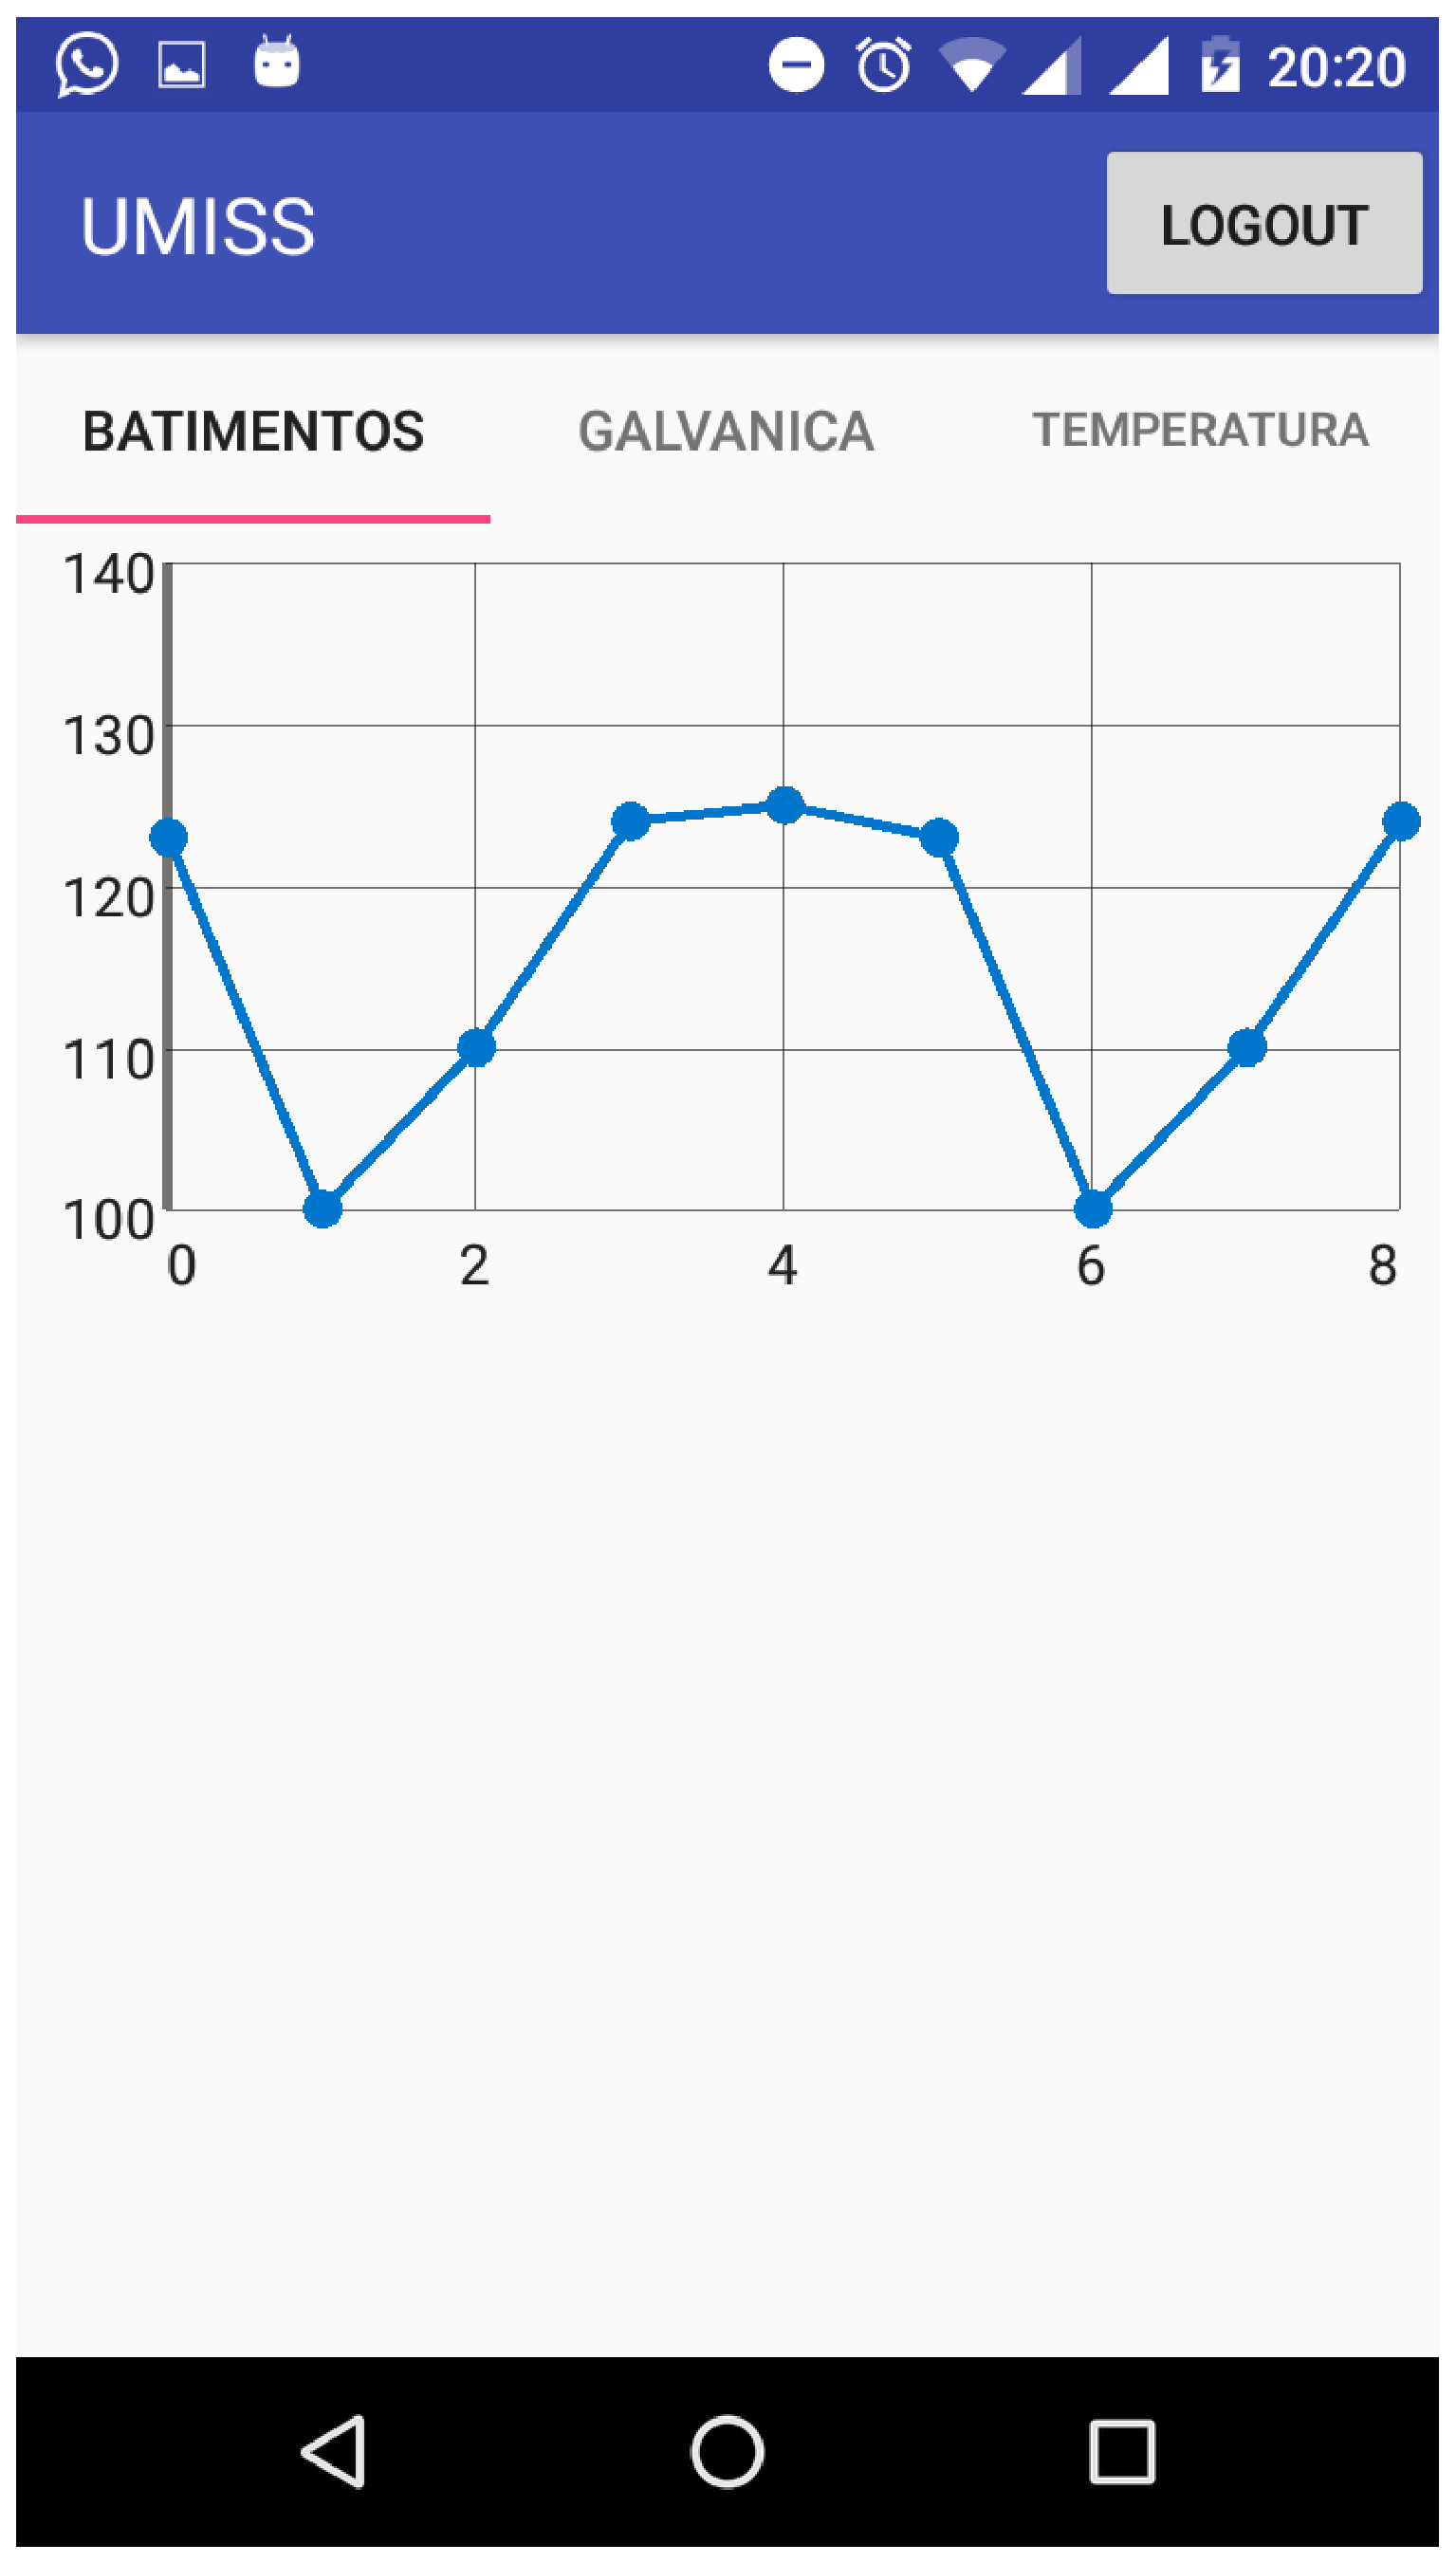
\includegraphics[scale=0.25]{figuras/android.eps}
    \end{center}
    \caption{Layout atual da tela principal do módulo Android.}
\end{figure}

\end{itemize}

